\section{Results}
\label{sec:results}

% NOTE: sources. Main numbers: paper_tables/T3_main_results.tex, paper_figures/*.csv. Tests, Holm-adjusted p-values, sensitivity analyses and the matched-baseline mitigation numbers: claim_audit_report.md (5,000 image-cluster bootstrap resamples, seed 42). T3, Fig 4 and Fig 9 use 2,000 stratified resamples, so their intervals differ slightly in the third decimal. Regenerate everything from one bootstrap configuration before submission.
% NOTE: \rad{} marks radiology-dependent statements. Radiology is affected by the duplicated-image issue (claim_audit_report.md, X1).
% NOTE: macros assumed: \SMHR, \CHR, \SRI, \PH{}, \rad{}.

This section reports the results in the order of the four questions posed in the Introduction. Section~\ref{subsec:res_ranking} gives the model-level ranking and the extent to which it is supported by the data. Section~\ref{subsec:res_sri} compares the domain-adapted models with the best general-purpose model in each modality. Section~\ref{subsec:res_modality} describes the dependence on modality, on the type of image and on the type of query. Section~\ref{subsec:res_transfer} examines the agreement of rankings across modalities, and Section~\ref{subsec:res_metrics} compares \SMHR{} with two published scores. Section~\ref{subsec:res_robust} reports the robustness of the main conclusions, and Section~\ref{subsec:res_mitigation} reports the mitigation experiments. All intervals are 95\% intervals from a bootstrap that resamples images, and not responses or claims, unless stated otherwise.

\subsection{Model ranking}
\label{subsec:res_ranking}

Table~\ref{tab:main} gives the \SMHR{} and \CHR{} of the twelve models, overall and by modality, and Figure~\ref{fig:ranking} shows the overall ranking with the bootstrap range of each rank. The \SMHR{} ranged from \PH{0.529} for Qwen2.5-VL to \PH{0.794} for LLaVA-Med. Five general-purpose models formed the lowest-\SMHR{} group, with values from \PH{0.529} to \PH{0.562}. Four of the remaining seven models are general-purpose (MiniCPM-V, Idefics3, Qwen2-VL and LLaVA-1.6, with values from \PH{0.580} to \PH{0.675}) and three are domain-adapted (HuatuoGPT-Vision \PH{0.691}, CheXagent \PH{0.748} and LLaVA-Med \PH{0.794}).

\begin{table*}[t]
\centering
\scriptsize
\begin{tabular}{lccccc}
\toprule
Model & Overall & Rad & Derm & Histo & Ophth \\
\midrule
\multicolumn{6}{l}{\textit{SMHR [95\% CI] (lower is safer)}} \\
\midrule
Qwen2.5-VL & 0.529 [0.524, 0.535] & 0.728 [0.720, 0.736] & 0.348 [0.338, 0.358] & 0.533 [0.522, 0.544] & 0.455 [0.441, 0.470] \\
Gemma3 & 0.532 [0.525, 0.539] & 0.633 [0.621, 0.645] & 0.461 [0.448, 0.473] & 0.575 [0.555, 0.594] & 0.465 [0.450, 0.480] \\
InternVL3 & 0.539 [0.533, 0.545] & 0.652 [0.645, 0.660] & 0.447 [0.434, 0.460] & 0.504 [0.490, 0.518] & 0.470 [0.456, 0.484] \\
Qwen3.5 & 0.549 [0.542, 0.556] & 0.675 [0.666, 0.684] & 0.496 [0.482, 0.510] & 0.482 [0.464, 0.500] & 0.416 [0.400, 0.431] \\
Qwen3-VL & 0.562 [0.556, 0.569] & 0.764 [0.757, 0.771] & 0.415 [0.401, 0.429] & 0.521 [0.507, 0.535] & 0.418 [0.403, 0.434] \\
MiniCPM-V & 0.580 [0.574, 0.586] & 0.619 [0.611, 0.626] & 0.533 [0.518, 0.546] & 0.646 [0.627, 0.664] & 0.442 [0.429, 0.454] \\
Idefics3 & 0.636 [0.630, 0.643] & 0.644 [0.635, 0.653] & 0.602 [0.590, 0.614] & 0.651 [0.634, 0.668] & 0.627 [0.609, 0.645] \\
Qwen2-VL & 0.643 [0.638, 0.648] & 0.828 [0.824, 0.834] & 0.435 [0.424, 0.447] & 0.564 [0.550, 0.579] & 0.571 [0.561, 0.581] \\
LLaVA-1.6 & 0.675 [0.669, 0.681] & 0.746 [0.737, 0.756] & 0.565 [0.552, 0.578] & 0.716 [0.703, 0.728] & 0.571 [0.556, 0.584] \\
HuatuoGPT-V$^{\dagger}$ & 0.691 [0.687, 0.695] & 0.827 [0.822, 0.833] & 0.574 [0.564, 0.585] & 0.631 [0.620, 0.641] & 0.564 [0.554, 0.574] \\
CheXagent$^{\dagger}$ & 0.748 [0.742, 0.755] & 0.826 [0.817, 0.834] & 0.629 [0.615, 0.643] & 0.736 [0.720, 0.751] & 0.727 [0.711, 0.742] \\
LLaVA-Med$^{\dagger}$ & 0.794 [0.790, 0.797] & 0.921 [0.917, 0.925] & 0.645 [0.634, 0.656] & 0.745 [0.737, 0.751] & 0.669 [0.663, 0.674] \\
\midrule
\multicolumn{6}{l}{\textit{CHR [95\% CI]: share of responses with a class 1 or 2 hallucination}} \\
\midrule
Qwen2.5-VL & 0.785 [0.778, 0.792] & 0.944 [0.937, 0.951] & 0.675 [0.658, 0.694] & 0.799 [0.780, 0.815] & 0.629 [0.616, 0.642] \\
Gemma3 & 0.731 [0.723, 0.740] & 0.873 [0.859, 0.886] & 0.744 [0.728, 0.762] & 0.544 [0.526, 0.563] & 0.690 [0.675, 0.705] \\
InternVL3 & 0.760 [0.752, 0.768] & 0.949 [0.942, 0.957] & 0.631 [0.610, 0.651] & 0.714 [0.694, 0.732] & 0.654 [0.640, 0.669] \\
Qwen3.5 & 0.773 [0.766, 0.781] & 0.880 [0.872, 0.888] & 0.750 [0.735, 0.766] & 0.634 [0.614, 0.654] & 0.788 [0.773, 0.802] \\
Qwen3-VL & 0.730 [0.722, 0.737] & 0.876 [0.867, 0.886] & 0.584 [0.567, 0.600] & 0.706 [0.687, 0.723] & 0.703 [0.685, 0.721] \\
MiniCPM-V & 0.715 [0.707, 0.723] & 0.922 [0.915, 0.929] & 0.635 [0.619, 0.654] & 0.539 [0.514, 0.563] & 0.675 [0.661, 0.688] \\
Idefics3 & 0.800 [0.793, 0.806] & 0.920 [0.911, 0.928] & 0.758 [0.746, 0.772] & 0.765 [0.748, 0.782] & 0.681 [0.670, 0.693] \\
Qwen2-VL & 0.797 [0.790, 0.804] & 0.948 [0.943, 0.954] & 0.693 [0.675, 0.711] & 0.751 [0.734, 0.769] & 0.727 [0.716, 0.739] \\
LLaVA-1.6 & 0.741 [0.733, 0.750] & 0.887 [0.876, 0.898] & 0.654 [0.637, 0.672] & 0.668 [0.647, 0.688] & 0.694 [0.681, 0.705] \\
HuatuoGPT-V$^{\dagger}$ & 0.806 [0.800, 0.812] & 0.970 [0.964, 0.976] & 0.675 [0.658, 0.692] & 0.782 [0.767, 0.797] & 0.722 [0.708, 0.737] \\
CheXagent$^{\dagger}$ & 0.719 [0.711, 0.727] & 0.765 [0.753, 0.777] & 0.723 [0.706, 0.740] & 0.769 [0.749, 0.788] & 0.561 [0.552, 0.571] \\
LLaVA-Med$^{\dagger}$ & 0.750 [0.742, 0.758] & 0.886 [0.874, 0.897] & 0.685 [0.667, 0.703] & 0.613 [0.592, 0.633] & 0.770 [0.760, 0.779] \\
\bottomrule
\end{tabular}
\caption{Core-run results for 12 VLMs on 3,500 images. Intervals are 95\% image-level bootstrap CIs (2,000 resamples, stratified by design stratum, seed 42); $^{\dagger}$ medical specialist. CHR = share of responses containing at least one fabrication or omission.}
\label{tab:main}
\end{table*}


\begin{figure}[t]
  \centering
  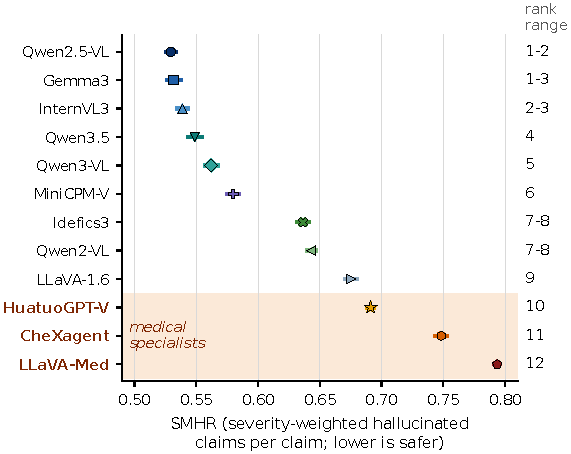
\includegraphics[width=\columnwidth]{paper_figures/fig02_smhr_ranking.pdf}
  \caption{\SMHR{} of 12 VLMs on 3,500 images (11,750 responses per model); lower is safer, and domain-adapted models are shaded. Bars are 95\% image-level bootstrap intervals (2,000 resamples, seed 42). The right-hand column gives the 95\% bootstrap range of each model's rank, so that models with overlapping ranges are not ordered.}
  \label{fig:ranking}
\end{figure}

The data support a coarse ordering and not a strict one. Of the 66 pairs of models, 63 have a paired difference whose interval excludes zero. The three exceptions are adjacent pairs: Qwen2.5-VL and Gemma3 (difference \PH{0.002}, interval \PH{$-0.006$ to $0.011$}), Gemma3 and InternVL3 (\PH{0.007}, \PH{$-0.002$ to $0.016$}) and Idefics3 and Qwen2-VL (\PH{0.007}, \PH{$-0.001$ to $0.015$}). Among the five leading models, the ten pairwise differences were tested with Holm correction. Qwen3-VL was separated from each of the other four, and Qwen3.5 was separated from Qwen2.5-VL and Gemma3 but not from InternVL3. Qwen2.5-VL, Gemma3 and InternVL3 were not separated from one another after correction. Qwen2.5-VL held the first rank in \PH{69\%} of resamples and Gemma3 in \PH{31\%}. An ordering within the first three models is therefore not supported, and the statement that can be made is that five general-purpose models formed the lowest group. Without the radiology images, Qwen2.5-VL ranked first (\SMHR{} \PH{0.428}) and Gemma3 fell to the fifth place \rad{}, which is a further reason not to rank within this group.

The \CHR{} ranged from \PH{0.715} to \PH{0.806} across models and was not correlated with the rank by \SMHR{} (Spearman $\rho = \PH{0.00}$). MiniCPM-V and CheXagent had the lowest \CHR{}, but the three lowest values (\PH{0.715} to \PH{0.730}) lie within sampling error of one another. The two metrics therefore answer different questions: the \CHR{} reports how often a response contains at least one fabrication or omission, whereas \SMHR{} reports the severity-weighted share of all claims. The number of claims extracted differs by a factor of about \PH{3.6} between models, from \PH{21,767} for LLaVA-Med to \PH{78,744} for Qwen3.5. Because \SMHR{} is a mean over claims, a model whose responses contain many correct claims can obtain a lower value without producing fewer serious errors, and the claim counts should be considered when the values are interpreted. The retrieval experiments in Section~\ref{subsec:res_mitigation} illustrate this effect.

Among the domain-adapted models, CheXagent and LLaVA-Med had the two highest \SMHR{} in every analysis. HuatuoGPT-Vision ranked tenth overall and eighth without the radiology images \rad{}, ahead of LLaVA-1.6 and Idefics3 in that analysis. The statement that the three domain-adapted models are the three worst models therefore does not hold in all analyses. It held in \PH{84\%} of random perturbations of the class weights by up to 30\%. The values for LLaVA-Med were obtained from responses of which a substantial share were truncated by a decoding defect; this is discussed in Section~\ref{subsec:res_sri}.

\subsection{Domain-adapted and general-purpose models}
\label{subsec:res_sri}

Figure~\ref{fig:sri} and Table~\ref{tab:sri} report the \SRI{} of each domain-adapted model in each modality. The reference is the general-purpose model with the lowest \SMHR{} in the modality and is held fixed in the bootstrap. It is MiniCPM-V for radiology, Qwen2.5-VL for dermatology, and Qwen3.5 for histopathology and ophthalmology. In ophthalmology Qwen3.5 (\PH{0.416}) and Qwen3-VL (\PH{0.418}) are not distinguishable, and Qwen3.5 had the lowest value in \PH{60\%} of resamples.

\begin{table}[t]
\centering
\small
\caption{Specialisation ratio index (\SRI) of the domain-adapted models, with 95\% image-level bootstrap intervals (2,000 resamples, reference model held fixed). A value above 1 indicates a higher \SMHR{} than the best general-purpose model in the modality. All twelve intervals exclude 1.}
\label{tab:sri}
\begin{tabular}{@{}lcccc@{}}
\toprule
Model & Radiology \rad{} & Dermatology & Histopathology & Ophthalmology \\
\midrule
HuatuoGPT-Vision & 1.34 [1.32, 1.36] & 1.65 [1.60, 1.70] & 1.31 [1.26, 1.37] & 1.36 [1.31, 1.41] \\
CheXagent & 1.34 [1.31, 1.36] & 1.81 [1.75, 1.87] & 1.53 [1.46, 1.59] & 1.75 [1.67, 1.82] \\
LLaVA-Med & 1.49 [1.47, 1.51] & 1.85 [1.80, 1.91] & 1.54 [1.49, 1.60] & 1.61 [1.55, 1.67] \\
\midrule
Reference model & MiniCPM-V & Qwen2.5-VL & Qwen3.5 & Qwen3.5 \\
\bottomrule
\end{tabular}
\end{table}

\begin{figure}[t]
  \centering
  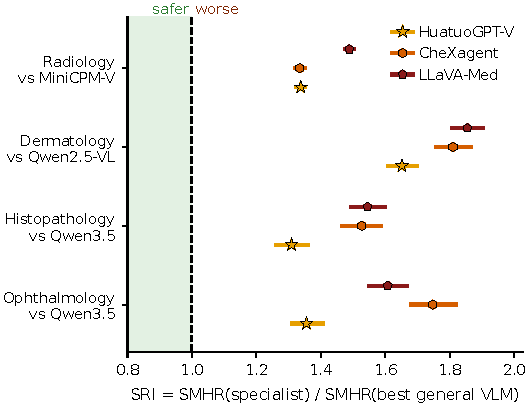
\includegraphics[width=\columnwidth]{paper_figures/fig04_specialization_paradox.pdf}
  \caption{\SRI{} of each domain-adapted model by modality. Values above 1 indicate that the model hallucinates more than the best general-purpose model named under each modality. Bars are 95\% image-level bootstrap intervals (2,000 resamples; reference model held fixed) over 3,500 images (1,200, 900, 800 and 600 per modality). The intervals of the three models overlap in several cells, and the models should not be ranked against each other from this figure.}
  \label{fig:sri}
\end{figure}

Each domain-adapted model had a higher \SMHR{} than the best general-purpose model in each of the four modalities. The \SRI{} ranged from \PH{1.31} to \PH{1.85}, the lowest lower bound of an interval was \PH{1.26}, and all twelve cells remained significant after Holm correction (adjusted $p = \PH{0.011}$, the smallest value attainable with the number of permutations used). The result was stable under the following changes.
\begin{itemize}
  \item Equal class weights: \SRI{} from \PH{1.30} to \PH{1.62}, with the lowest lower bound \PH{1.27}.
  \item Random perturbation of each class weight by up to 30\%, 2,000 draws: all twelve cells remained above 1 in every draw, with a minimum of \PH{1.13}.
  \item Selection of the reference model on one random half of the images and measurement on the other half, 1,000 splits: all twelve cells remained above 1 in every split.
  \item Removal of the radiology images: the nine remaining cells are unchanged. On the \PH{113} radiology images with distinct content the \SRI{} ranged from \PH{1.48} to \PH{1.77} \rad{}.
  \item Random flips of up to \PH{13\%} of the claim-level judge labels: all twelve cells remained above 1.
\end{itemize}

The result is a comparison of each domain-adapted model with the best of nine general-purpose models. It does not show that the domain-adapted models are worse than every general-purpose model. HuatuoGPT-Vision had a lower \SMHR{} than \PH{one} general-purpose model in radiology and in dermatology and than \PH{three} in histopathology and in ophthalmology; CheXagent had a lower \SMHR{} than one general-purpose model in radiology and than none in the other modalities; LLaVA-Med had a lower \SMHR{} than none. The comparison also does not isolate the effect of medical adaptation. The three domain-adapted models differ from the general-purpose models in parameter count, in architecture and in the date of release, and the design contains no base--specialist pairs. CheXagent was developed for chest radiography, so that its values in the other three modalities measure in part the transfer of a chest radiograph model to other domains. The ratio of \SMHR{} to the reference should therefore be read as a descriptive measurement for the checkpoints and the protocol examined here.

The \SRI{} of LLaVA-Med is an upper bound. In the core run, a decoding defect caused \PH{about one third} of the LLaVA-Med responses to begin in mid-sentence.
% NOTE: the audit gives 32% of responses; figure_manifest.md gives 50% of Q1 responses. State the basis of the percentage. On the responses that were regenerated with the corrected decoder the \SMHR{} was \PH{0.728}, against \PH{0.791} for the same items in the core run, a reduction of about \PH{8\%}. The \SRI{} values of LLaVA-Med stay above 1 under this correction.
% NOTE: confirm whether the core run is rerun or both numbers are reported; the core-run numbers are the ones in T3.

\subsection{Dependence on modality, image type and query}
\label{subsec:res_modality}

Figure~\ref{fig:modality} shows the \SMHR{} of each model in each modality and the composition of the flagged claims by class. Radiology had the highest \SMHR{} for 10 of the 12 models, and this held also on the \PH{113} radiology images with distinct content \rad{}. Dermatology had the lowest \SMHR{} for 9 of the 12 models, with a bootstrap range of 6 to 10 models. Modality and model identity each accounted for roughly 40\% to 50\% of the variance in the 48 cell-level values of \SMHR{}. This is a descriptive decomposition of the cells and not a test.

\begin{figure*}[t]
  \centering
  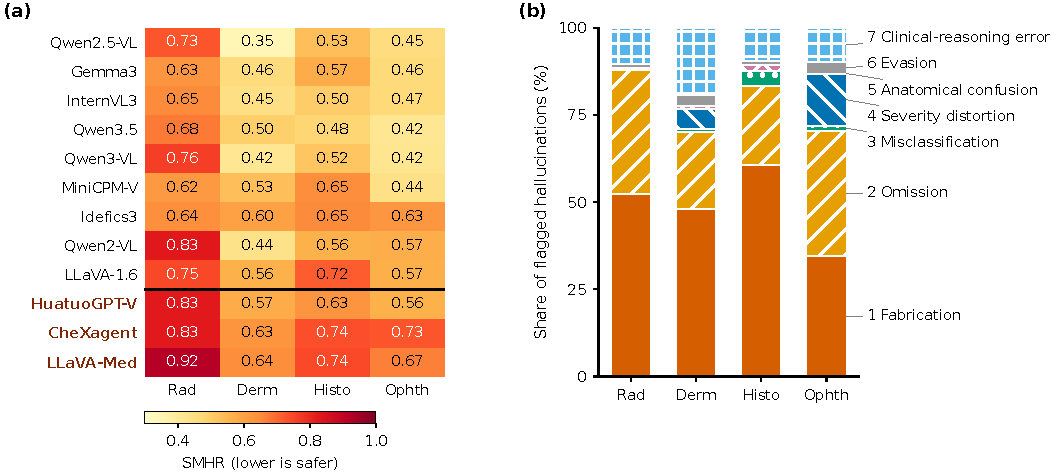
\includegraphics[width=\textwidth]{paper_figures/fig03_modality_fingerprints.pdf}
  \caption{(a) \SMHR{} by model and modality; the intervals of each cell are given in the source data. (b) Share of flagged claims by hallucination class within each modality, pooled over the 12 models (353,625 flagged claims and omissions). The thick line separates general-purpose models (above) from domain-adapted models (below).}
  \label{fig:modality}
\end{figure*}

The composition of errors differs between modalities. Fabrication and omission together accounted for \PH{88\%} of the flagged claims in radiology \rad{}, \PH{83\%} in histopathology, \PH{71\%} in ophthalmology and \PH{70\%} in dermatology. Fabrication was the largest class in radiology, dermatology and histopathology (\PH{52\%}, \PH{48\%} and \PH{61\%}), and omission was the largest in ophthalmology (\PH{36\%}). Clinical reasoning error accounted for \PH{19\%} of the flagged claims in dermatology and \PH{10\%} in each of the other modalities, and severity distortion for \PH{15\%} in ophthalmology and \PH{6\%} in dermatology. Anatomical confusion, evasion and misclassification each accounted for no more than \PH{5\%} in any modality. The class-specific labels are not validated against independent annotation (Section~\ref{sec:validation}), so that this composition is descriptive.

The interpretation of the \SMHR{} depends on how much of each class can be checked against the available ground truth. In radiology, \PH{93\%} of the weighted error comes from classes with full coverage by the labels, although the radiology labels are subject to the image issue \rad{}. In dermatology the share is \PH{57\%}, in ophthalmology \PH{50\%}, and in histopathology none, because essentially all of the weighted error (\PH{99.9\%}) comes from classes that can be checked only partially, fabrication and omission alone accounting for \PH{89\%}: the PatchCamelyon half of the histopathology images has binary tumour labels only. The \SMHR{} in histopathology is therefore a proxy for the hallucination rate and not a complete measurement of it.

Normal images did not uniformly draw more hallucination than abnormal ones. Across the four modalities and twelve models, the difference in \SMHR{} between the normal and the abnormal strata for the first three queries had either sign, with the exception of ophthalmology, where the \SMHR{} on normal images was lower for all twelve models (mean difference \PH{$-0.31$}). The false-premise query had a clear effect on normal images. The \SMHR{} for the fourth query was higher than for the first three queries for \PH{10 of the 12} models, lower for one (Qwen3-VL) and unchanged for one (HuatuoGPT-Vision), with a mean difference of \PH{0.14}. Figure~\ref{fig:normal} in the appendix gives the underlying values. This differs from the finding of HalluCXR that normal radiographs drew the most severe hallucinations \citep{wang2026hallucxr}, which was obtained for chest radiographs only and with a different grading scheme, and the present data do not permit a direct comparison.

\subsection{Agreement of rankings across modalities}
\label{subsec:res_transfer}

The rankings of the twelve models by \SMHR{} in dermatology, histopathology and ophthalmology were positively correlated (Figure~\ref{fig:transfer} in the appendix). The Spearman correlation was \PH{0.81} for dermatology and histopathology (permutation $p = \PH{0.002}$, Holm-adjusted $p = \PH{0.013}$), \PH{0.77} for histopathology and ophthalmology (\PH{0.005}, \PH{0.024}) and \PH{0.66} for dermatology and ophthalmology (\PH{0.022}, \PH{0.088}). The last of these does not remain significant after correction. Among the nine general-purpose models alone the correlations were smaller and none was significant (\PH{0.62}, \PH{0.60} and \PH{0.33}). The cross-modality association therefore reflects in large part the fact that the domain-adapted models and the weakest general-purpose models rank poorly in every modality. With three domain-adapted models, a correlation of the \SRI{} values across modalities cannot reach a two-sided $p$ below \PH{0.33}, and it is not reported.

The correlations between radiology and the other modalities were \PH{0.21}, \PH{0.27} and \PH{0.49}, none of them significant. On the \PH{113} radiology images with distinct content they were \PH{0.36}, \PH{0.55} and \PH{0.69}. The first set is an artefact of the duplicated images, and the second rests on a small number of images. Whether rankings transfer to and from radiology could not be assessed in this study \rad{}.
% NOTE: Fig 6 labels its Holm p-values from a t-based test (0.008, 0.074, 0.017); the audit uses permutation p-values (0.013, 0.088, 0.024). Use one convention.

\subsection{Comparison with published scores}
\label{subsec:res_metrics}

The \SMHR{} was compared with the risk-weighted score of CREST \citep{crest2025medrxiv} and with the MediHall Score \citep{chen2024medhallmark}, both computed on the same classified claims. The comparison is shown in Figure~\ref{fig:concordance} in the appendix. The \SMHR{} and CREST were positively rank-correlated across the twelve models (Spearman $\rho = \PH{0.64}$, permutation $p = \PH{0.03}$, 95\% interval \PH{0.07 to 0.90} by Fisher transformation). The CREST values were confined to a narrow interval (\PH{2.67 to 2.86} on a scale from 1 to 3), so that the agreement rests on small differences. Seven of ten model--modality cells in which the two scores diverge by more than one standard deviation were stable in more than \PH{90\%} of the bootstrap resamples, and three lay at the threshold. The \SMHR{} and the MediHall Score ranked the twelve models identically ($\rho = \PH{-1.00}$). This agreement is expected from the construction of the two scores, since both are weighted error rates over the same classified claims and their class weights correlate with $r = \PH{0.95}$, and it should not be read as independent confirmation. The unweighted error rate alone correlates with the \SMHR{} at $\rho = \PH{0.965}$. On these data the \SMHR{} therefore does not order the models differently from a MediHall-style score. Its distinct contributions are the claim as the unit of analysis, the explicit omission class, and the cross-modality reference provided by the \SRI{}.

\subsection{Robustness}
\label{subsec:res_robust}

Three sources of uncertainty not captured by the image-level bootstrap were examined.

\paragraph{Class weights.} Under equal weights and under 200 random perturbations of up to 30\% the ranking of the twelve models was essentially unchanged (Spearman $\rho \geq \PH{0.88}$ against the ranking with the assumed weights). The weights themselves were not elicited from clinicians, so that this analysis establishes only the stability of the conclusions with respect to the weights.

\paragraph{Judge labels.} All values depend on one local model that extracts and judges claims (Section~\ref{sec:setup}). The only component independent of this model is the omission count of the first layer, which accounts for between \PH{25\%} and \PH{42\%} of the weighted error. Re-running the judge on identical text changed \PH{1.1\%} of the strict and \PH{2.8\%} of the claim-level labels, and the labels produced by the core pipeline and by the later pipeline for the same responses differed for \PH{2.1\%} and \PH{11.3\%} of \PH{195} responses. Symmetric random flips of 3\% and 5\% of the claim-level labels changed none of the main conclusions. At 13\% the identity of the two leading models changed. Systematic bias of the judge, for example towards outputs of models of the same family, was not assessed, and the evaluated set contains four models of the Qwen family.

\paragraph{Sampling.} The core run used one sample per image and query at temperature 0.1. Across four distinct decoding settings, the \SMHR{} of a single model varied by between \PH{0.022} (Qwen2.5-VL) and \PH{0.077} (HuatuoGPT-Vision), which exceeds the differences of \PH{0.002} to \PH{0.010} within the first three models. Stochasticity can therefore change the order within the leading group. It cannot remove the gap of \PH{0.13} to \PH{0.26} between the five leading models and the domain-adapted models.

\subsection{Mitigation}
\label{subsec:res_mitigation}

Two inference-time strategies were compared on a subset of 500 images and five models: retrieval-augmented prompting and contrastive decoding. Fine-tuning was planned and not carried out. Both strategies were run with greedy decoding. The benchmark baseline is the response from the core run, generated by sampling at temperature 0.1. Because a change from sampling to greedy decoding can alter \SMHR{} by itself, each strategy is also compared with a matched greedy baseline from the calibration experiment. The matched baseline exists only for the items on which the greedy response stated a confidence, which is \PH{1,489}, \PH{1,179}, \PH{1,499} and \PH{1,385} of about 1,670 items for Qwen2.5-VL, LLaVA-1.6, CheXagent and HuatuoGPT-Vision, respectively; for LLaVA-Med the corrected greedy rerun was used. Decoding alone moved the \SMHR{} of LLaVA-1.6 by \PH{$-0.046$}, an interval excluding zero, and that of Qwen2.5-VL by \PH{$-0.011$}.

\begin{table*}[t]
\centering
\footnotesize
\caption{Change in \SMHR{} under retrieval-augmented prompting (RAG) and contrastive decoding (CD) on a 500-image subset, against the benchmark baseline (temperature 0.1) and a matched greedy baseline. Entries are the difference [95\% paired image-level bootstrap interval], with the Holm-adjusted $p$-value in parentheses (families of 10 tests per baseline). $^{\dagger}$ domain-adapted model. The subset includes radiology images affected by the image issue \rad{}.}
\label{tab:mitigation}
\begin{tabular}{@{}lcccc@{}}
\toprule
& \multicolumn{2}{c}{RAG} & \multicolumn{2}{c}{CD} \\
\cmidrule(lr){2-3}\cmidrule(lr){4-5}
Model & vs benchmark & vs matched greedy & vs benchmark & vs matched greedy \\
\midrule
Qwen2.5-VL & $-0.028$ [$-0.046$, $-0.011$] (0.015) & $-0.018$ [$-0.034$, $-0.001$] (0.26) & $-0.003$ [$-0.021$, $+0.016$] (1.00) & $+0.009$ [$-0.009$, $+0.027$] (1.00) \\
LLaVA-1.6 & $-0.042$ [$-0.061$, $-0.021$] (0.003) & $+0.041$ [$+0.021$, $+0.060$] (0.010) & $-0.085$ [$-0.105$, $-0.065$] (0.001) & $-0.031$ [$-0.053$, $-0.008$] (0.048) \\
HuatuoGPT-V$^{\dagger}$ & $+0.004$ [$-0.011$, $+0.019$] (1.00) & $-0.011$ [$-0.028$, $+0.005$] (0.96) & $-0.025$ [$-0.040$, $-0.010$] (0.015) & $-0.035$ [$-0.051$, $-0.020$] (0.001) \\
CheXagent$^{\dagger}$ & $+0.026$ [$+0.005$, $+0.048$] (0.12) & $+0.011$ [$-0.013$, $+0.035$] (1.00) & $-0.041$ [$-0.068$, $-0.015$] (0.028) & $-0.052$ [$-0.081$, $-0.022$] (0.010) \\
LLaVA-Med$^{\dagger}$ & $+0.003$ [$-0.010$, $+0.014$] (1.00) & $+0.003$ [$-0.010$, $+0.014$] (1.00) & $-0.005$ [$-0.019$, $+0.009$] (1.00) & $-0.005$ [$-0.019$, $+0.009$] (1.00) \\
\bottomrule
\end{tabular}
\end{table*}

Table~\ref{tab:mitigation} gives the results. Contrastive decoding gave the lowest \SMHR{} for four of the five models, and the reduction was reliable against the matched baseline for three of them: CheXagent ($-0.052$), HuatuoGPT-Vision ($-0.035$) and LLaVA-1.6 ($-0.031$). For LLaVA-Med and Qwen2.5-VL it was indistinguishable from the baseline. The reduction for HuatuoGPT-Vision was the only effect that held against both baselines and with and without the radiology images ($-0.025$ against the benchmark baseline and $-0.035$ against the matched baseline; $-0.050$ and $-0.062$ without radiology \rad{}). Without radiology, contrastive decoding increased the \SMHR{} of CheXagent by \PH{0.048} to \PH{0.056} (Holm-adjusted $p = \PH{0.05}$ to \PH{0.08}), so that its benefit for this model depends on the radiology images \rad{}.

Retrieval-augmented prompting did not lower \SMHR{} consistently. Against the benchmark baseline it appeared to lower it for Qwen2.5-VL and LLaVA-1.6, but against the matched greedy baseline the change for Qwen2.5-VL was not significant after correction, and for LLaVA-1.6 the \SMHR{} was higher by \PH{0.041}. The apparent gain for LLaVA-1.6 was concentrated in items on which the greedy response states no confidence and for which no matched label exists. On exactly the items that have one, the effect against the benchmark baseline was \PH{$-0.006$} [\PH{$-0.027$}, \PH{$+0.016$}]. For CheXagent the increase against the benchmark baseline was not significant after correction. Without the radiology images, retrieval increased the \SMHR{} of LLaVA-Med by \PH{0.037} (Holm-adjusted $p = \PH{0.010}$) \rad{}. In a direct comparison, contrastive decoding gave a lower \SMHR{} than retrieval for LLaVA-1.6, CheXagent and HuatuoGPT-Vision (Holm-adjusted $p \leq \PH{0.002}$), retrieval gave a lower value for Qwen2.5-VL ($+0.025$ in favour of retrieval, $p = \PH{0.015}$), and the two were tied for LLaVA-Med.

The \SMHR{} does not capture a second effect of retrieval. The share of responses that contain a fabrication or omission (\CHR{}) increased under retrieval for four of the five models: by \PH{0.12} for LLaVA-1.6, \PH{0.08} for HuatuoGPT-Vision, \PH{0.05} for CheXagent and \PH{0.03} for LLaVA-Med, with all four intervals excluding zero. For Qwen2.5-VL the increase of \PH{0.020} [\PH{$-0.003$}, \PH{$+0.042$}] was not distinguishable from zero. Retrieved text lengthened the answers and added correct claims, which can leave the \SMHR{} flat or lower it while more responses contain at least one serious error. A decrease in \SMHR{} under retrieval should not be read as a decrease in the number of harmful responses.

For the specialisation analysis, the mean \SRI{} over the twelve cells was \PH{1.401} for the benchmark baseline, \PH{1.516} for the matched greedy baseline, \PH{1.474} with retrieval and \PH{1.406} with contrastive decoding. Contrastive decoding reduced the mean \SRI{} against the matched greedy baseline by \PH{0.110} [\PH{0.039}, \PH{0.183}], and it did not change it against the benchmark baseline. Retrieval did not detectably change it. Neither strategy removed the gap between domain-adapted and general-purpose models.

\begin{figure}[t]
  \centering
  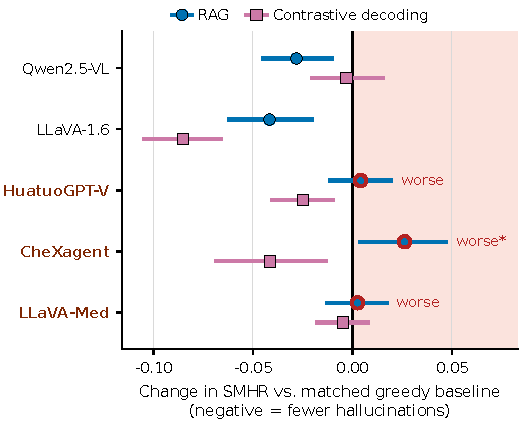
\includegraphics[width=\columnwidth]{paper_figures/fig09_mitigation.pdf}
  \caption{Change in \SMHR{} relative to the benchmark baseline for retrieval-augmented prompting and contrastive decoding (five models, 1,659 to 1,678 paired image--query responses on a 500-image subset). Bars are 95\% paired image-level bootstrap intervals (2,000 resamples). Outlines mark strategies that increase \SMHR{}.}
  \label{fig:mitigation}
\end{figure}
% NOTE: Fig 9 and T4 were produced against the benchmark baseline; the manifest caption calls it a matched greedy baseline, which is incorrect. Regenerate Fig 9 against the matched greedy baseline, or keep this caption.

\subsection{Calibration of stated confidence}
\label{subsec:res_calibration}

The calibration of stated confidence was examined for five models under six decoding configurations on the same subset (Figure~\ref{fig:calibration} in the appendix). Under the strict correctness label, accuracy was between \PH{12\%} and \PH{28\%} while the mean stated confidence was between \PH{52\%} and \PH{91\%}. The expected calibration error was between \PH{0.50} and \PH{0.73}, and at least \PH{75\%} of the gap came from overconfident bins. The three greedy configurations produced identical responses, so that four configurations are independent. Across these four, the ordering of the five models by calibration error was stable (mean pairwise Spearman $\rho = \PH{0.90}$, 95\% interval \PH{0.83 to 0.95}, with the image as the unit of resampling), and HuatuoGPT-Vision was the worst-calibrated model in every configuration. With one prompt and five models, this result shows that the ordering is insensitive to the decoding setting. It does not show that calibration is a property of the model weights.
